\begin{figure*}[h]                                                           
 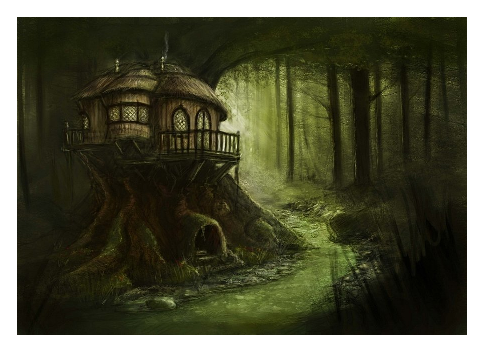
\includegraphics[width=\linewidth]{./media/images/article_one_splash}%
  \small{\textsc{\\ Human perception spans} all our senses and sensibilities.
    Here are a few ways to codify your readers' experience. (Photo: \href{https://www.deviantart.com/tomallica}{\textsc{Tom Walker)}}}
  \label{fig:bridge}%                                                 
\end{figure*}                                                                
\begin{quotation} 
\noindent\color{Sepia}{\scriptsize{\textit{\textbf{“One's
          destination is never a place, but a new way of seeing things.” }}}}\\[2mm]
   \hfill\color{Sepia}{\scriptsize{\textendash Henry Miller}}
\end{quotation} 

\section{museums for the mind}

% ** Story Layer
% *** Room Descriptions
% **** Wikipedia summaries useful here
% **** Multiple Responses for area descriptions
% *** Leave Messages
% *** Arrival Message
% *** Travel Description
% *** Narrator
\lettrine[lines=3]{\color{BrickRed}O}{\enspace ne} of the joys of a good work of Interactive Fiction is the feeling
you get when you interact with the parser on something that you know probably
isn't part of the core for furthering the story but pleasantly discover that
your inquiry works anyway. Even if your interlocutors don't inspect every detail
of their surroundings, just knowing that he is touring a world crafted with care
goes a long way toward immersion.
\marginpar{
  \tiny{\textit{Taking the extra effort and polish to detail your world}}
}
A fleshed out world also, in a practical
sense, implicitely tells the interlocutor that not every object is significant.
This makes the reader have to understand the \textit{solution} the author is
trying to convey as the discovery may be had only through careful thought and
not through, ``Oh, here's a set of keys--these \textit{must} be important.'' A key to a work focused on immersion, I believe, is a world where the author has taken the time to respond intellegently to reasonable inquiries by the player. 

I garner the following factors important to give the reader a sense of immersion:

\begin{itemize}
  \item{Responses for all senses (touch, smell, etc.)}
\item{Differing descriptions based on direction of travel}
\item{Triggered, geography independent narrative}
\item{Multiple responses to the same command}
  \item{Leaving area messages based on conditions}
  \item{Arriving area messages based on conditions}
  \end{itemize}

\marginpar{\vspace{2mm}
  \tiny{\textit{A systematic approach to further your long term story goals}}
}

Fortunately, there are techniques that can help lighten the burden. Developing a systematic approach, at least during the planning phase, can help further your efforts and reduce the feeling that your remaining work is overwhelming.

\subsection{together we stand}
The first and most powerful technique, if possible, is to get help. Make a call
to the Interactive Fiction forums calling for help in areas you may not be
strong. In my case, I am both a good IF architect and writer but my writing is
slow. Someone else may be a good writer but finds ``slaving away'' building the
world model a task that is simply ``beneath'' their artistic talents.
\marginpar{
  \tiny{\textit{Talent wins games, but teamwork and intelligence win championships.}}
}
I, on the other hand, am a facilitator who craves giving artists the ability to
provide the audience with a world model who's prose is constantly fresh,
complete with varying responses based on the direction they're looking, varying
descriptions each time, decorative scenes, and atmosphere. I find the little
things not necessarily adding to the core of the work's message but
\marginpar{\vspace{2mm}
  \tiny{\textit{An ounce of detail is worth a pound of immersion.}}
}
furnishing the world with just a little extra detail immensely
satisfying.  The writer and I are a match made in heaven. The writer is
presented with a beautifully templated world model\textemdash all they need to do is fill in the blanks. I benefit because I can focus on the architecture and each components' relationship to one another.

\section{three layers of interaction}
\marginpar{\vspace{2mm}
  \tiny{\textit{A layered approach.}}
}If we take a work at face value to be focused on the narrative then it makes sense to find a way to weave the narrative in with the world model. This is the difference between a work that the interlocutor \textit{reads} and a work that he \textit{hacks through} looking for clues.


Let's break the work down into three layers, from the lowest to the highest:
\begin{itemize}
  \item{The Reference Layer}
  \item{The World View Layer}
  \item{The Story Layer}
\end{itemize}


\subsection{reference layer}
The reference layer provides the interlocutor with background information about
your world model to be looked up as needed. Several reference models are possible, anything from a notebook carried by the player, a computer terminal in the work, or even spinning rings as in Orson Well's \textit{The Time Machine}. The Reference Layer may even be a physical book or PDF distributed with the work.

Whatever form the factual reference layer takes it's purpose is to enrich the world model and to provide background and orientation to help the reader's success in the work.
\marginpar{\vspace{2mm}
  \tiny{\textit{The reference layer provides a segue to build cognitive world knowledge.}}
}
I don't want to confuse matters, but the reference layer also includes
descriptions of objects and areas after the initial examination/visit. The work
is structured to first give a "flowery" description of an object, for example,
but after that the factual layer takes over and provides a ``clinical'' view of
the scene. You've already weaved the significance of the given object in story form on first review. After this the interlocutor is familiar with this objects relationship in the world space and wishes to concentrate on the practical matter of deciphering the object's meaning in relation to achieving his goals.

\begin{centering}
\includegraphics[width=\textwidth]{./media/images/room_examine.png}
\end{centering}

\subsection{world view layer}
\noindent Moving up from the reference layer is the world view layer. This includes area/object descriptions, the interlocator's sense (sight, smell, touch, etc.) descriptions, and atmospheric spice sprinkled throughout the work.
\marginpar{\vspace{-2.5mm}
  \tiny{\textit{The world view layer grounds the reader in the world model.}}
}
Thousands of pages are written on this topic. The overarching theme is generally this: keep your descriptions sharp, brief and (by design) relevant. Recall that we've broken our work down into three distinct layers. We'll interweave literate prose in this World View Layer in the next layer up, that is, the Story Layer.

\begin{itemize}
  \item{Refined Prose for the initial view, factual view afterward}
  \item{Descriptions dependent on incoming direction}
  \item{Multiple descriptions to reduce tedium}
\end{itemize}
Mechanically, pointing a text summerizer at Wikipedia to boil down complex descriptions of an area to just a few sentances goes a long way to lighten the writer's burden. Place the summarizer's descriptions in your flowchart (outlined below). From here you flesh out the descriptions in your final work. Doing this goes a long way to not feeling like finishing the work is an insurmountable task.

\subsection{story layer}
\label{sec:story_layer}
This literary layer weaves the narrative with the world view layer. It's purpose is to bring narrative to the work--to make your story read like prose. The story layer also can help guide the interlocutor with hints.

\reversemarginpar
\marginpar{\vspace{2mm}
  \tiny{\textit{The narrator fills real\textendash time gaps in the reader's
      thinking, helping him to achieve the next crest of the story.}}
}

I implemented the story layer through three methods in \textsc{tads}. The first is the "initial description" feature, the second by the use of travel messages, and the third a special 'narrator' character who, while not physically existing in the model, injects prose into the work. The narrator is triggered by event state changes.

\normalmarginpar
\marginpar{\vspace{-40mm}
  \includegraphics[width=\linewidth]{./media/images/prop}
  \tiny{\textit{The reader is greeted with ancient proportions in
      The Acropolis (Photo: \href{https://commons.wikimedia.org/w/index.php?curid=156815}{\textsc{joseph kürschner}}}})
}

Here's an example of using refined prose for the initial view:

\begin{quote}
\small{
Propylaea Gateway

Reddish, golden light bathes the tops of the massive walls fortressed against the violet sky.  The contrast of light and shadow sharply mirrors
the angles of the opposing walls relative to the rising sun.  Below the sun's grasp lies softer, luminous blue light making angled pockets of
shadow.  Dew lightly covers the ground and continues up the walls where it glistens as tiny, fractured rainbows above the shadowed relief.  The
air is fresh and slightly chilly with an awakening smell of moist clay.

Beyond the wall's opening to the northeast lie a wide flight of steps rising 40 meters and stretching roughly 25 meters wide.  The steps end to
meet a large six-columned Doric facad at the top.

A scholarly man somewhere in his mid-sixties reads from a scroll nearby.  His calm posture looks to Xantius as he's patiently waited for a
thousand years.  He wears a white robe with a red sash draped around his
shoulders to his mid-section.
} % end small
\end{quote}

\noindent Okay, noting earth shattering here\textendash IF writers have used this
technique for years. You get to exercise your writing chops and, most
importantly, the reader is greeted with engaging prose. Your
descriptions speak directly to the reader. If we've ``gotten out of the way''
and formed a direct conduit to the reader we've done our job.

Let's move from here northeast up the Proplyaea's steps through the archway of
the fortressed wall. Initially, the interlocutor reads thus:

\begin{quote}
  \small{
Propylaea Steps

Moving higher, Xantius's footsteps echo from the steps' sides, where he is now about halfway up.  The Proylaea steps rise impressively before
Xantius, stretching across his entire field of view; roughly 100 men could stand shoulder-to-shoulder spanning the steps' width.  The stairs are
divided into three sections by virtue of their varying grades: finer, longer front-to-back cuts in the center shouldered by shallower, steeper
cuts on either side.  The steps continue upwards to a landing.  A narrower and steeper set of stone steps cut inset to the ridge on Xantius's
right.

\textbf{[The Interlocutor moves further up the steps and then back down.]}

Propylaea Steps

The Proylaea steps continue their descent to the Acropolis outer walls before Xantius, stretching his entire field of view.  The steps run higher
above and behind you to a landing A small flight of steps cut into the steps' border wall lead off to your left (South).

\textbf{[The Interlocutor moves further down the steps and then back up again.]}

Propylaea Steps

Xantius moves up the Propylaea steps, this time on the right side where the grade of the steps are steeper.  ``I wonder why they made the outside
grade of the steps steeper than the inside?  Was it so merchants could make it easier for supplies to be delivered by cart to the Acropolis?'' he
thinks, approaching the stone steps leading in from Xantius's right.  Before him the Propylaea steps rise to the upwards to the West Porch

\textbf{> look}

Propylaea Steps

The Propylaea steps rise at roughly a six per cent grade from the southwest to northeast, running roughly 300 meters from the Propylaea to the
stairs' top to the West Porch.

  }
\end{quote}
  
There's a lot going on here. The interlocutor first gets quality descriptive
prose when first encountering an area. When he returns from the area from a
different direction the description adapts itself to the reader's opposite
vantage point. When combined with varying prose dependent on direction of travel
and the environmental messages I mentioned above you breath life into your
story.
\marginpar{\vspace{2mm}
  \tiny{\textit{Varying responses keeps the world model interesting.}}
}
Also, we've varied the description outlining the reader's travel with, ``\ldots moves
up the Propylaea steps, this time on the right side where the grade of the steps
are steeper.'' These small details go a long way toward immersion and reduces tedium.

Notice the last passage, when the reader enters \textbf{\textit{look}}. We know that he's looking for factual
information about his surroundings. A ``just the facts'' description, indeed, is
exactly what we give him (The Propylaea steps rise at roughly six percent grade\ldots). The \textit{look} command is an indicative command as
it indicates what type of response he's looking for.

\subsubsection{all work and no play}
\label{play}

We can leverage the concept of indicative commands by recognizing when the
interlocutor tries things that are just plain silly.

\marginpar{\vspace{2mm}
  \tiny{\textit{Never taking yourself too seriously.}}
}
For example, when the reader is standing in the Propylaea Gateway from the example above all his senses
are available to him. He can smell the air, smell the wall, etc. None of these
commands are silly, per se, except when he tries to \textbf{\textit{lick the wall}}:

\begin{quote}
  \small{
    Propylaea Gateway
    
    \textbf{> lick wall}
    
Xantius extends his tongue and leans close to the wall.  "This is crazy," Xantius
thought, pausing for a moment to consider how he might appear to perplexed on-lookers.
"C'mon, " he godes himself, "go ahead, go ahead and lick it, I 'double-dog' dare you!"
Moving again closer, Xantius's outstretched tongue contacts the rough wall, making
tacid contact pressing to "full-on" docking.  He imagines himself viewed from the side,
his tongue and the wall's permiations now inversely mirroring each other in perfect
relief.

Xantius's laranyx lets out a half cough as the rest of his pie hole is engaged with
this ridiculous show of machismic servitude.  Xantius textures the invading, finely-
particled nip of marble and limestone on his tonque and, in a twist he hadn't
considered, the outter perimeter of his mouth.  His moist breath sucks some of the
wall's material back into the openings surrounding the axis of his acrid folly.

"Congratulations, Xantius," he thought, "you're a hero."

A little eternity passes before Xantius pulls his geology-coated tongue away from the
wall.  He presently gets right to making several paultry facial expressions as he
tries to dislodge the grit from his mouth\textemdash to end the grinding sound of sand emanating
from inside his skull, broadcasting his displeasure in the process.
} %end small
\end{quote}

\noindent Here we ``break the fourth wall'' giving the reader the idea that we've been
thoughtful designing our world and a break from the challenge intrinsic in the
experience.

\subsection{narration, morgan freeman style}

Here is an example of enhancing the story through a narrator as mentioned on
page \pageref{sec:story_layer}. If the protagonist doesn't bother to say hello
to the scholarly man wearing the sash this will happen (please excuse the
terrible writing):
\begin{quote}
  \small{
    Propylaea Gateway
    
   \textbf{> ne}

Each of Xantius's senses vie for his attention as he pieces together meaning of the
scene before him.  He moves slowly, noticing the "crunch, crunch" of the paultered
ground under his feet turning to a paddled beat on the marble steps.  With his footing
tentatively stepping upward on the Propylaea steps, he raises his gaze upward,
naturally straining his neck higher as he sizes up the ascent's rising to the six-
columned Doric facad marking the entrance of the Acropolis proper.

"What kind of civilization builds a place like this?"  Xantius asks himself, "If such
a place on earth hadn't existed prior to time of the Acropolis's conception, who
envisioned the city...what genius created it?"

Pausing, Xantius breathes in the the dense, moist air breezing in from the nearby
Medditerranian Sea.

Xantius suddenly realizes, "I hadn't gotten that man's name!  I have many questions, to not
sieze the opportunity to speak with him again is to betray it."
    } %end small
\end{quote}

\noindent When Xantius travels after having met the man, Xantius is greated with the
varied travel/description prose as described above plus this bit (again, please
excuse the corny dialog):

\begin{quote}
  \small{
    Propylaea Gateway
    
    \textbf{> ne}
    
   \textbf{[Story travel/description dialog]}

   ``I just met Socrates.  The.  Socrates.  Xantius bolted at the idea. I have so many
questions to ask him!''

\ldots
  }%end small
\end{quote}

\section{tying loose ends}
In the next issue of \textit{Discover's Digest} I'll include more specific
examples and code snippets for applying the layering techniques we discussed above.
% In Chapter \ref{ch:implement} on page \pageref{ch:implement} I'll include structure and code snippets for implementation details.